\documentclass{article}
\usepackage[utf8]{vietnam}
\usepackage{amsmath}
\usepackage{systeme,mathtools}
\usepackage{pgfplots}


\title{MaSSP Lecture 2 (part 2)}
\author{Kieu Anh Le}
\date{July 2019}

\begin{document}

\maketitle

\section{Review toán nền tảng:}
\subsection{Linear function}
Hàm tuyến tính F: $X\overset{f}{\rightarrow}Y$\\
hay Y = f(X)
\begin{itemize}
    \item Trường hợp 1: $X\in R^d; Y\in R$ \\
    => Y = $a^T.x +b  (a\in R^d, b \in R)$ 
    \item $y = a^T.x + b = \dot{a}^T.\dot{X}$\\
    Trong đó: $\dot{a} = \begin{bmatrix}
            b\\
            a
            \end{bmatrix}$  ;
            $\dot{X} = \begin{bmatrix}
            1\\
            X
            \end{bmatrix}$
    \item Trường hợp 2: $X\in R^d; Y\in R^k$ \\
    => Y= $W_x + b (W \in R^{kxd})$ W là 1 ma trận\\
    Có thể viết: $Y=\dot{W}.\dot{X}$
    Trong đó: $\dot{W} = \begin{bmatrix}
            w_1\\
            ... \\
            w_{d+1}
            \end{bmatrix}$  ;
            $\dot{X} = \begin{bmatrix}
            1\\
            ...\\
            X
            \end{bmatrix}$
    
    
\end{itemize}

         
\subsection{Non-linear function}
\begin{itemize}
    \item Để cố định 1 khoảng giá trị cho output -> \textbf{Dùng hàm sigmoid}\\
    VD: $y \in R -> \sigma(y) \in (0,1) \\
    => 2\sigma(y) - 1 \in (-1,1)$
    \item Để loại bỏ những giá trị không mong muốn (VD: loại bỏ giá trị <0, chỉ lấy phần dương) \\
    -> Dùng hàm ReLU: max(0,1)
    \item Softmax Function: Là hàm để tính xác suất của nhiều giá trị 
\end{itemize}

\section{Softmax Regression:}
\subsection{Softmax Function:}
Từ hàm sigmoid: $\sigma (y) = \sigma \begin{bmatrix}
    `       y_1\\
            ...\\
            y_k
            \end{bmatrix}
            = \begin{bmatrix}
    `       \sigma (y_1)\\
            ...\\
            \sigma (y_k)
            \end{bmatrix}$ \\
=> Normalize: $\frac{\sigma (y_1)}{\sum_{i=1}^{k} \sigma (y_i)}$\\
Với p=softmax(y) => \\ $0\leq p_i \leq 1$ \\ $\sum_{i=1}^{k} p_i=1$ \\
=> Tác dụng: Sử dụng để chuyển đổi từ vector tọa độ thành vector xác suất
\subsection{Bài toán Softmax Regression:}
\subsubsection{Unified Framework:}
\begin{figure}[ht]

\begin{center}

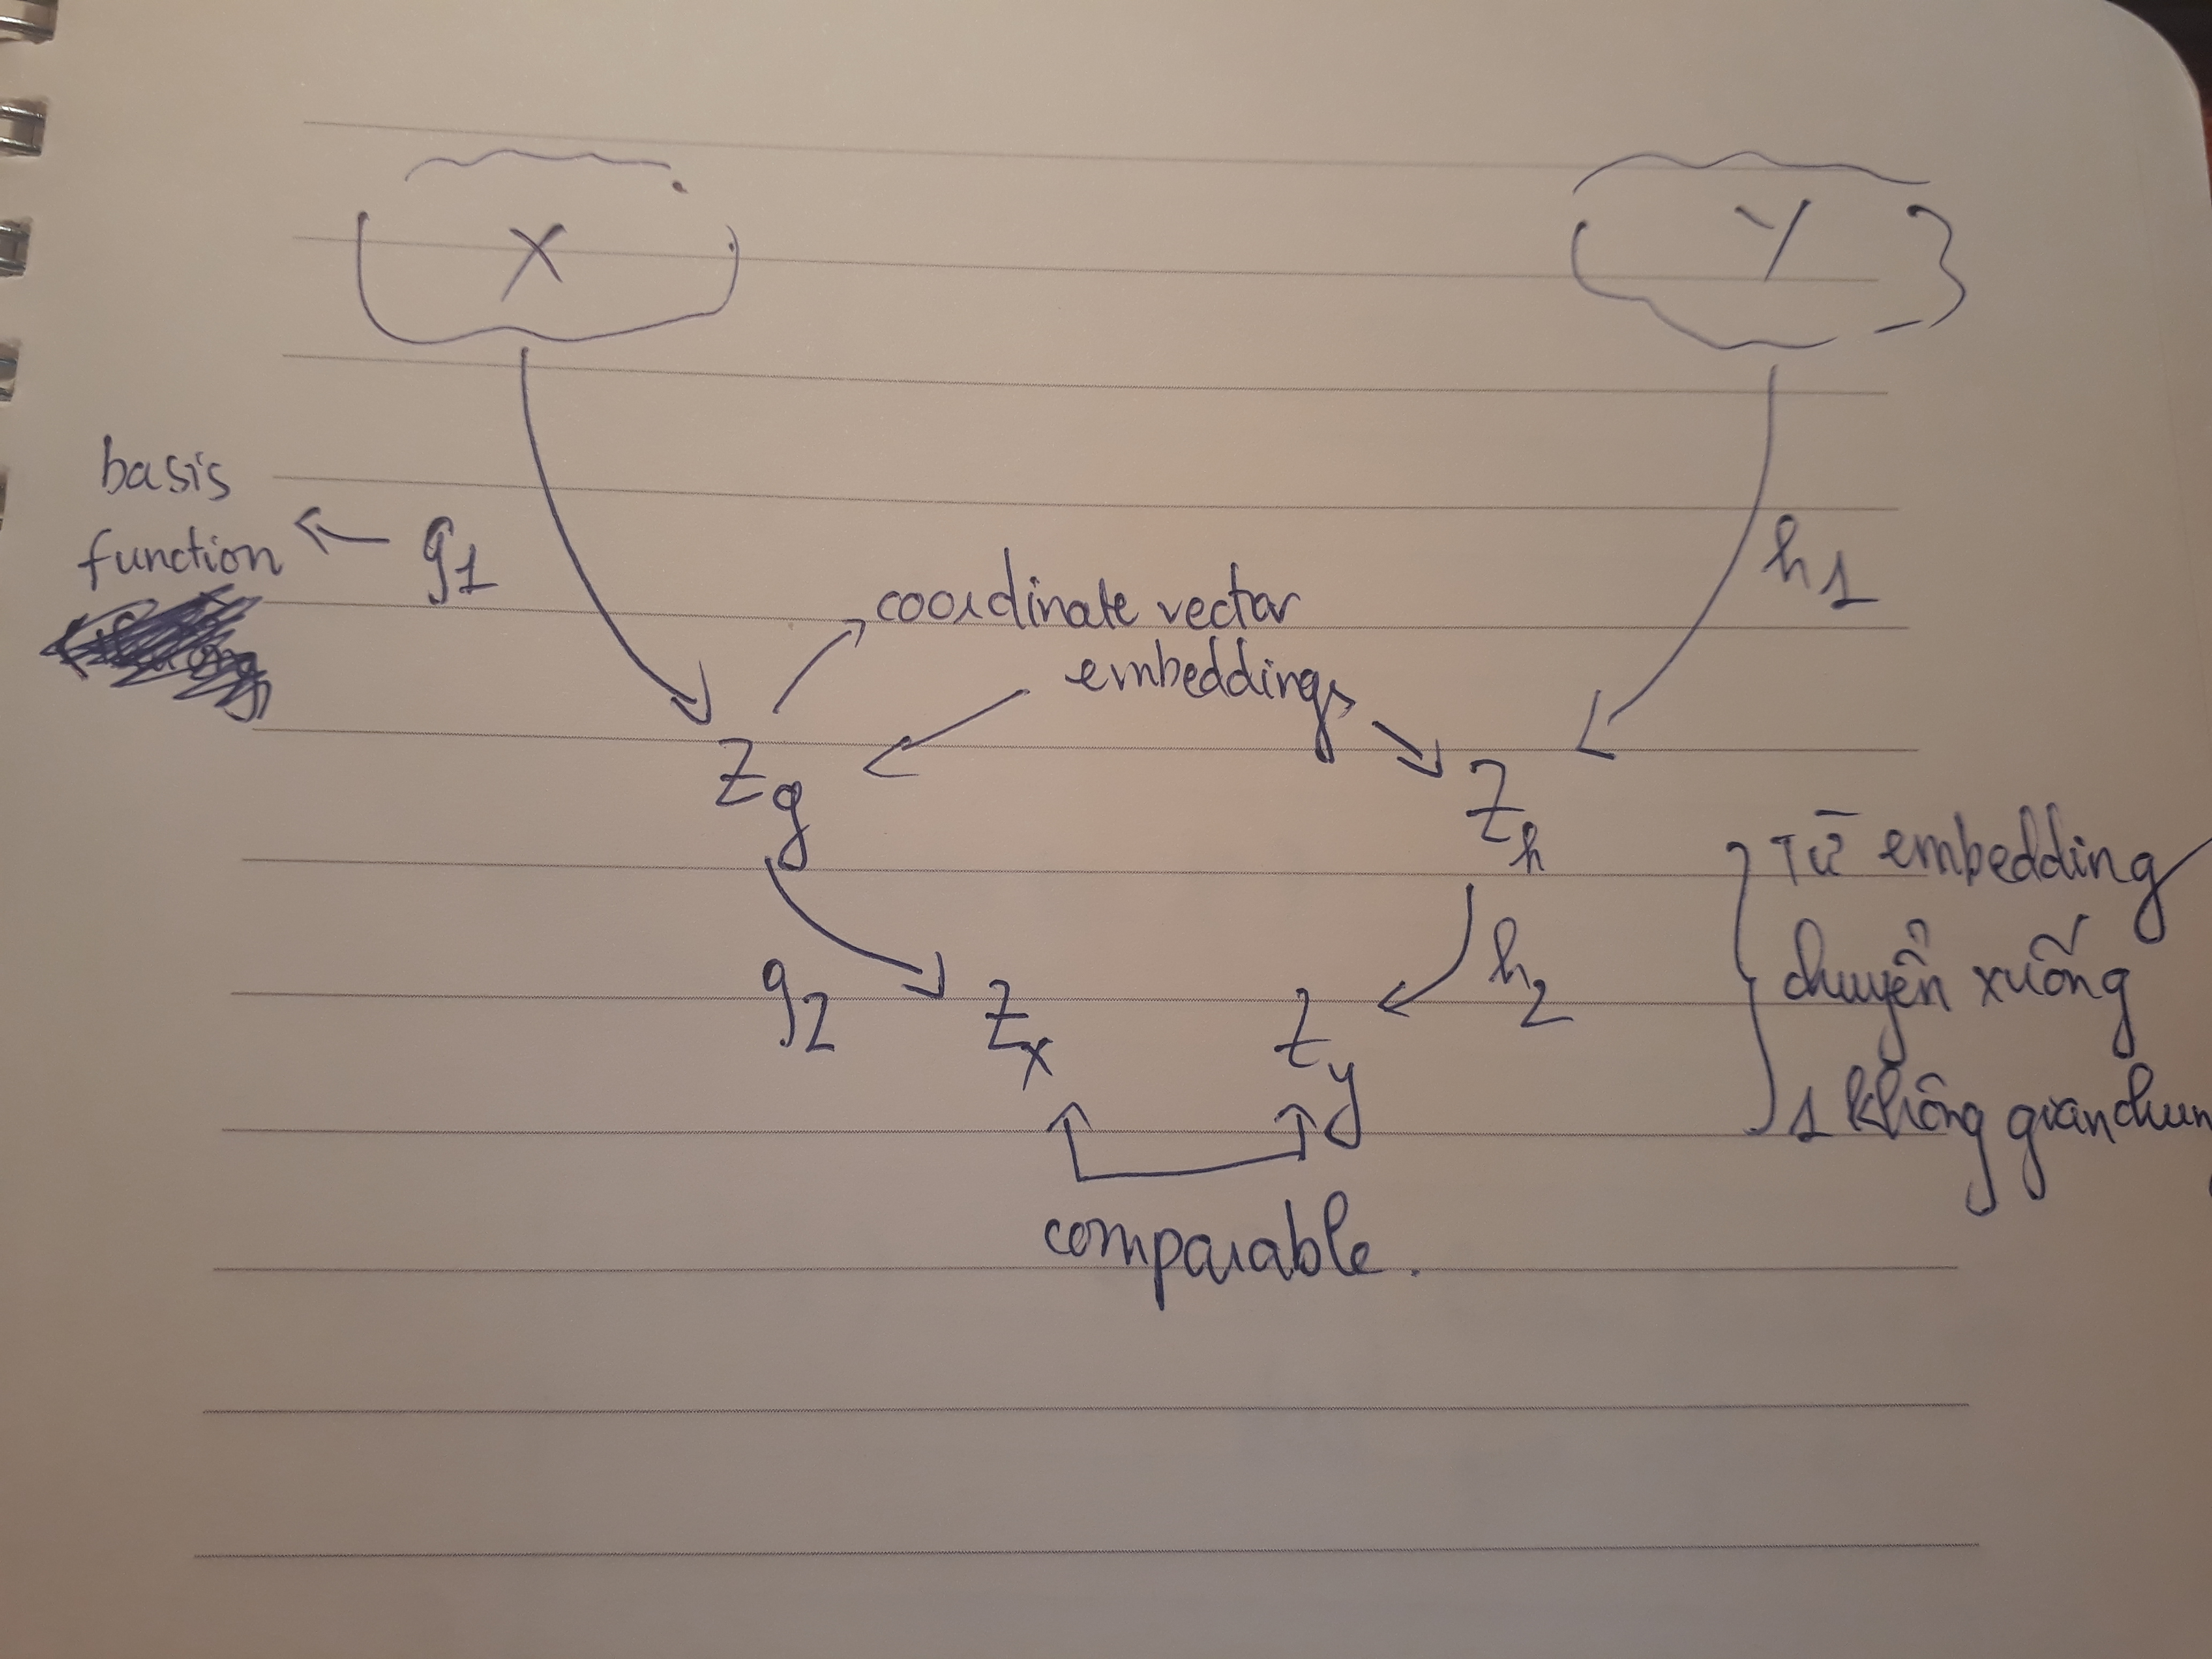
\includegraphics[scale=0.1]{20190703_001236}\\

\end{center}

\caption{Unified Framework}

\end{figure}

- Basis function g1: dùng linear function \\
- g2: dùng non-linear function (sigmoid, ReLU, ...) -> Có tác dụng trích xuất ra $Z_x$ có thể so sánh được với $Z_y$\\

\subsubsection{Giải thích bài toán Softmax Regression:}
\begin{figure}[ht]

\begin{center}

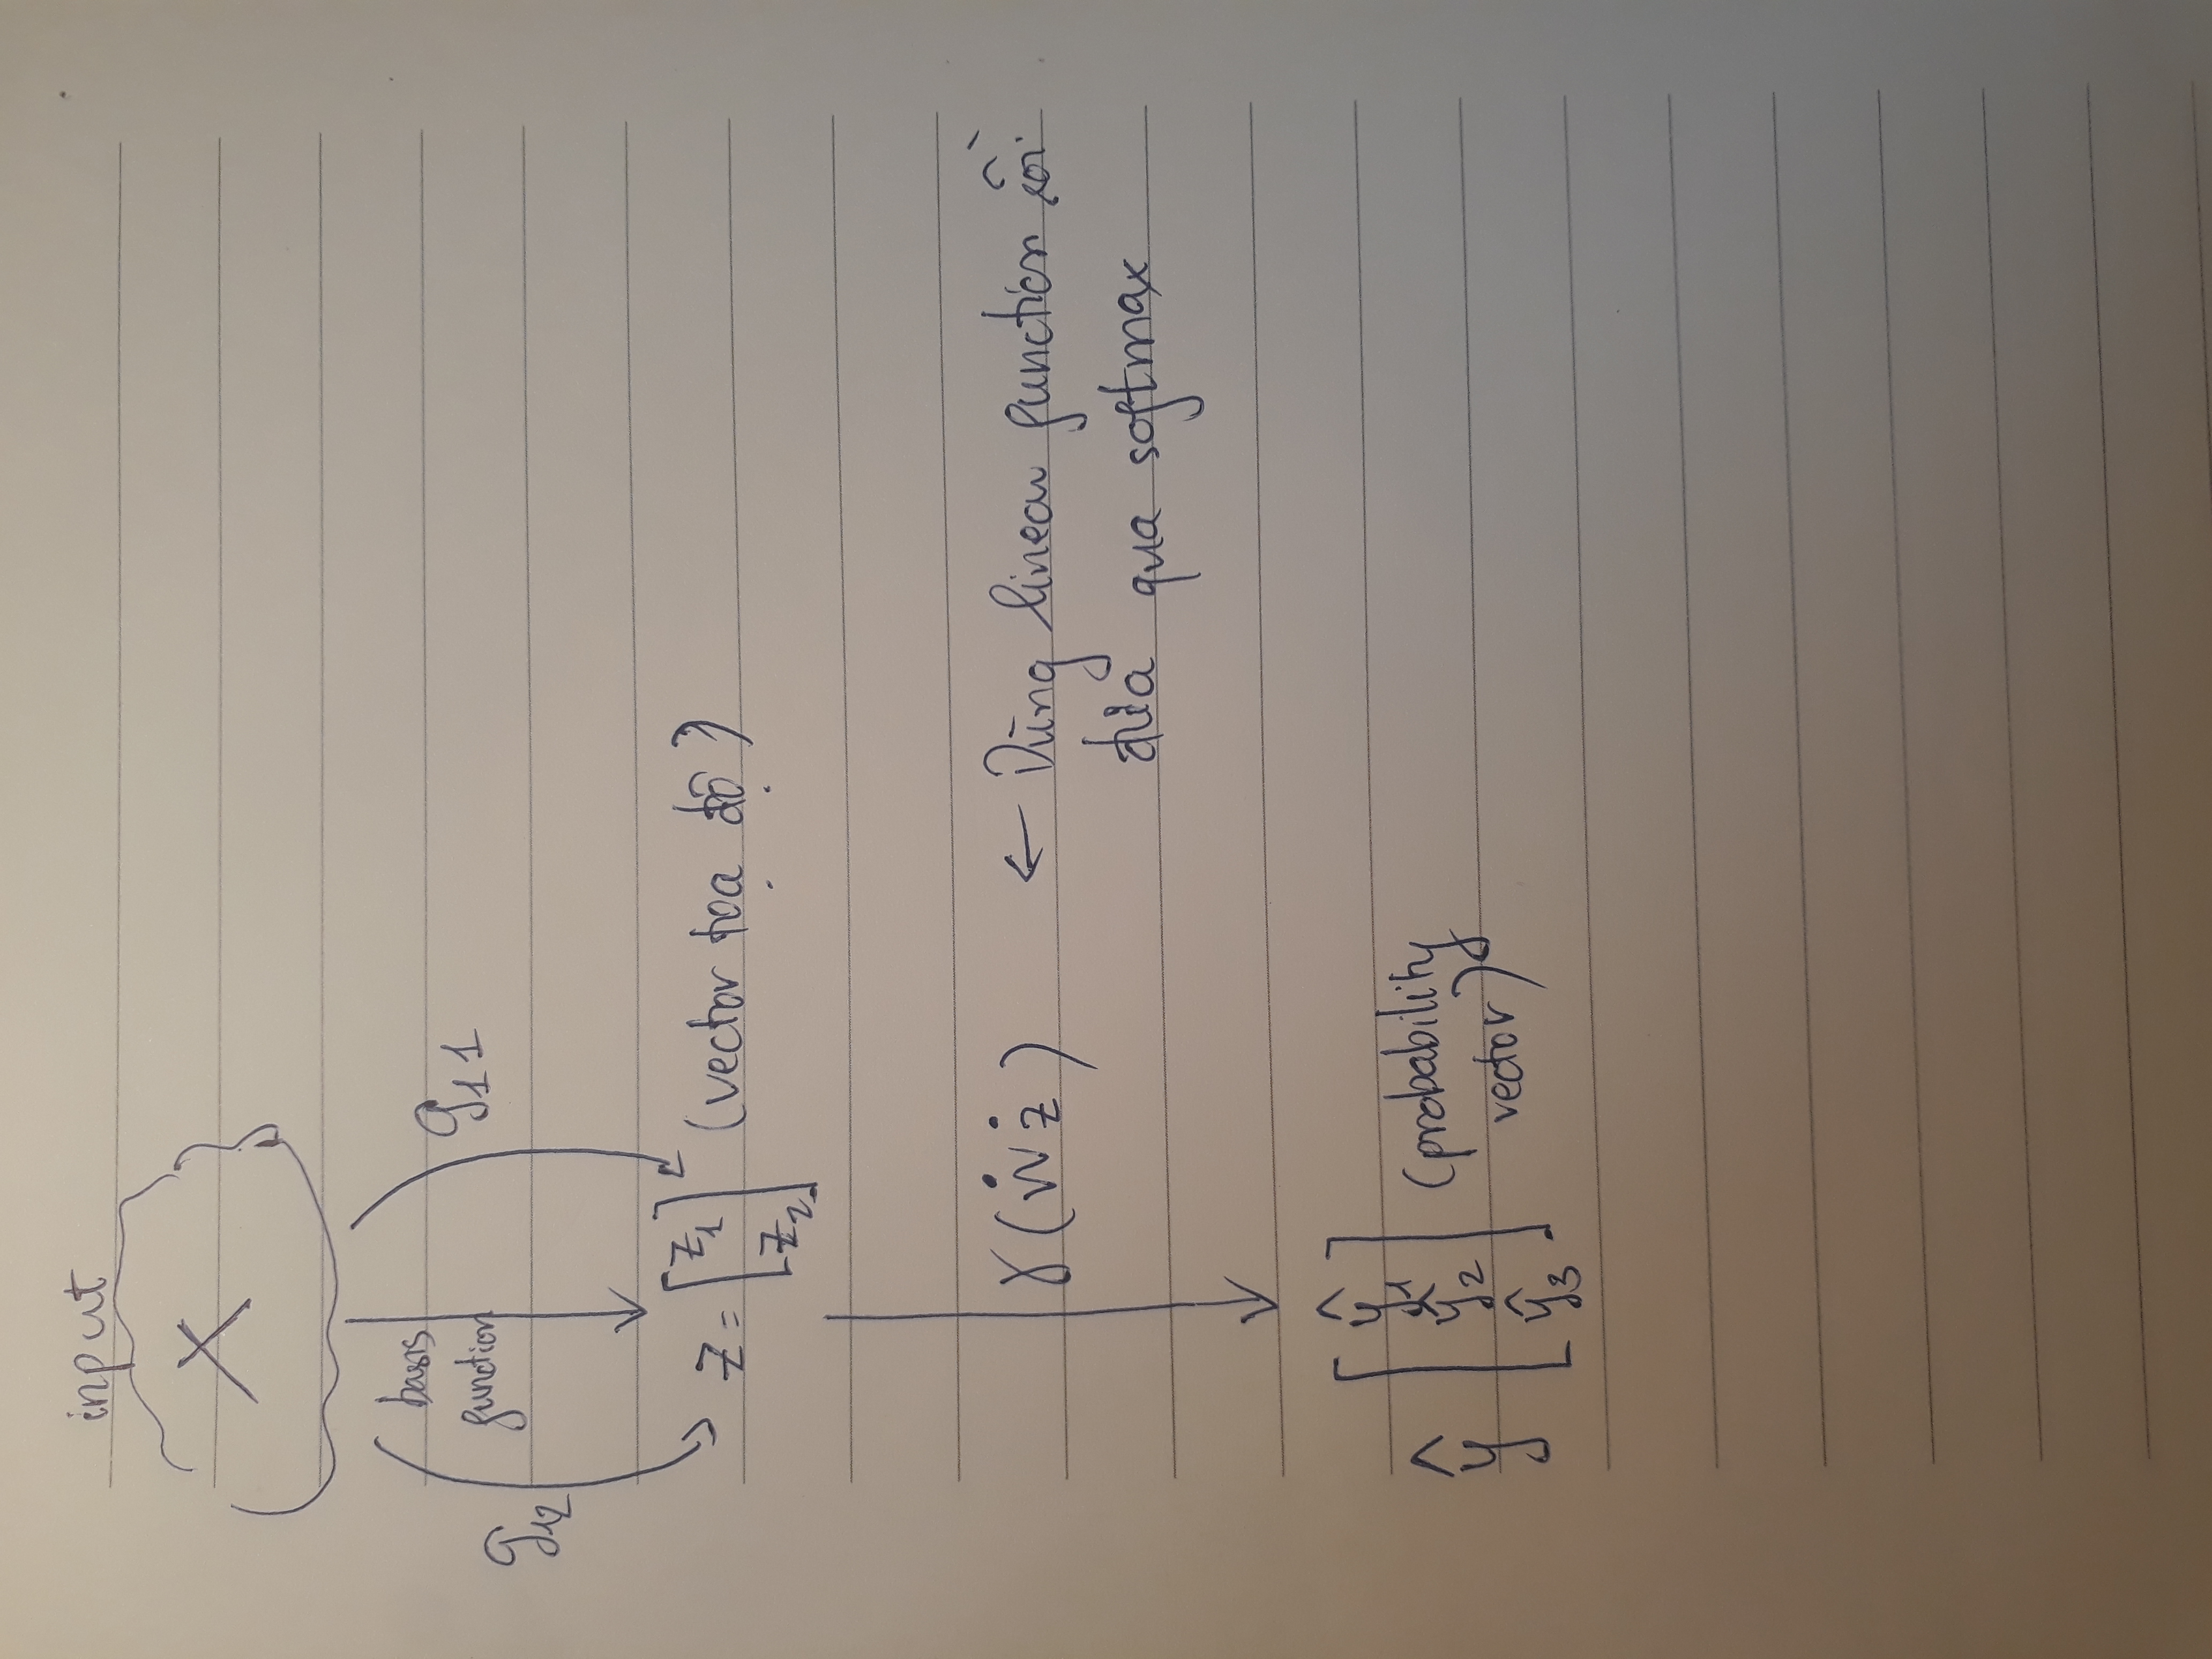
\includegraphics[scale=0.1]{20190703_001318.jpg}\\

\end{center}

\caption{Unified Framework - Softmax Regression}

\end{figure}
-  Mục tiêu: Vẽ đường chia cắt (decision boundary) những phần dữ liệu thuộc 3 class khác nhau  => Tie-breaking: Tìm tập hợp những điểm mà probability của 2 class bằng nhau (không tính được argmax của $\hat{y}_i$\\
- Cách tính xác suất lớn nhất: argmax $\hat{y}_i$, i=1->k

\section{Multi-layer Perceptron}
Bài toán: Vẽ những đường cong để phân chia các class dữ liệu không phân chia được bằng đường thẳng (linearly non-separable)\\
=> Cần dùng non-linear function 
\begin{figure}[ht]

\begin{center}

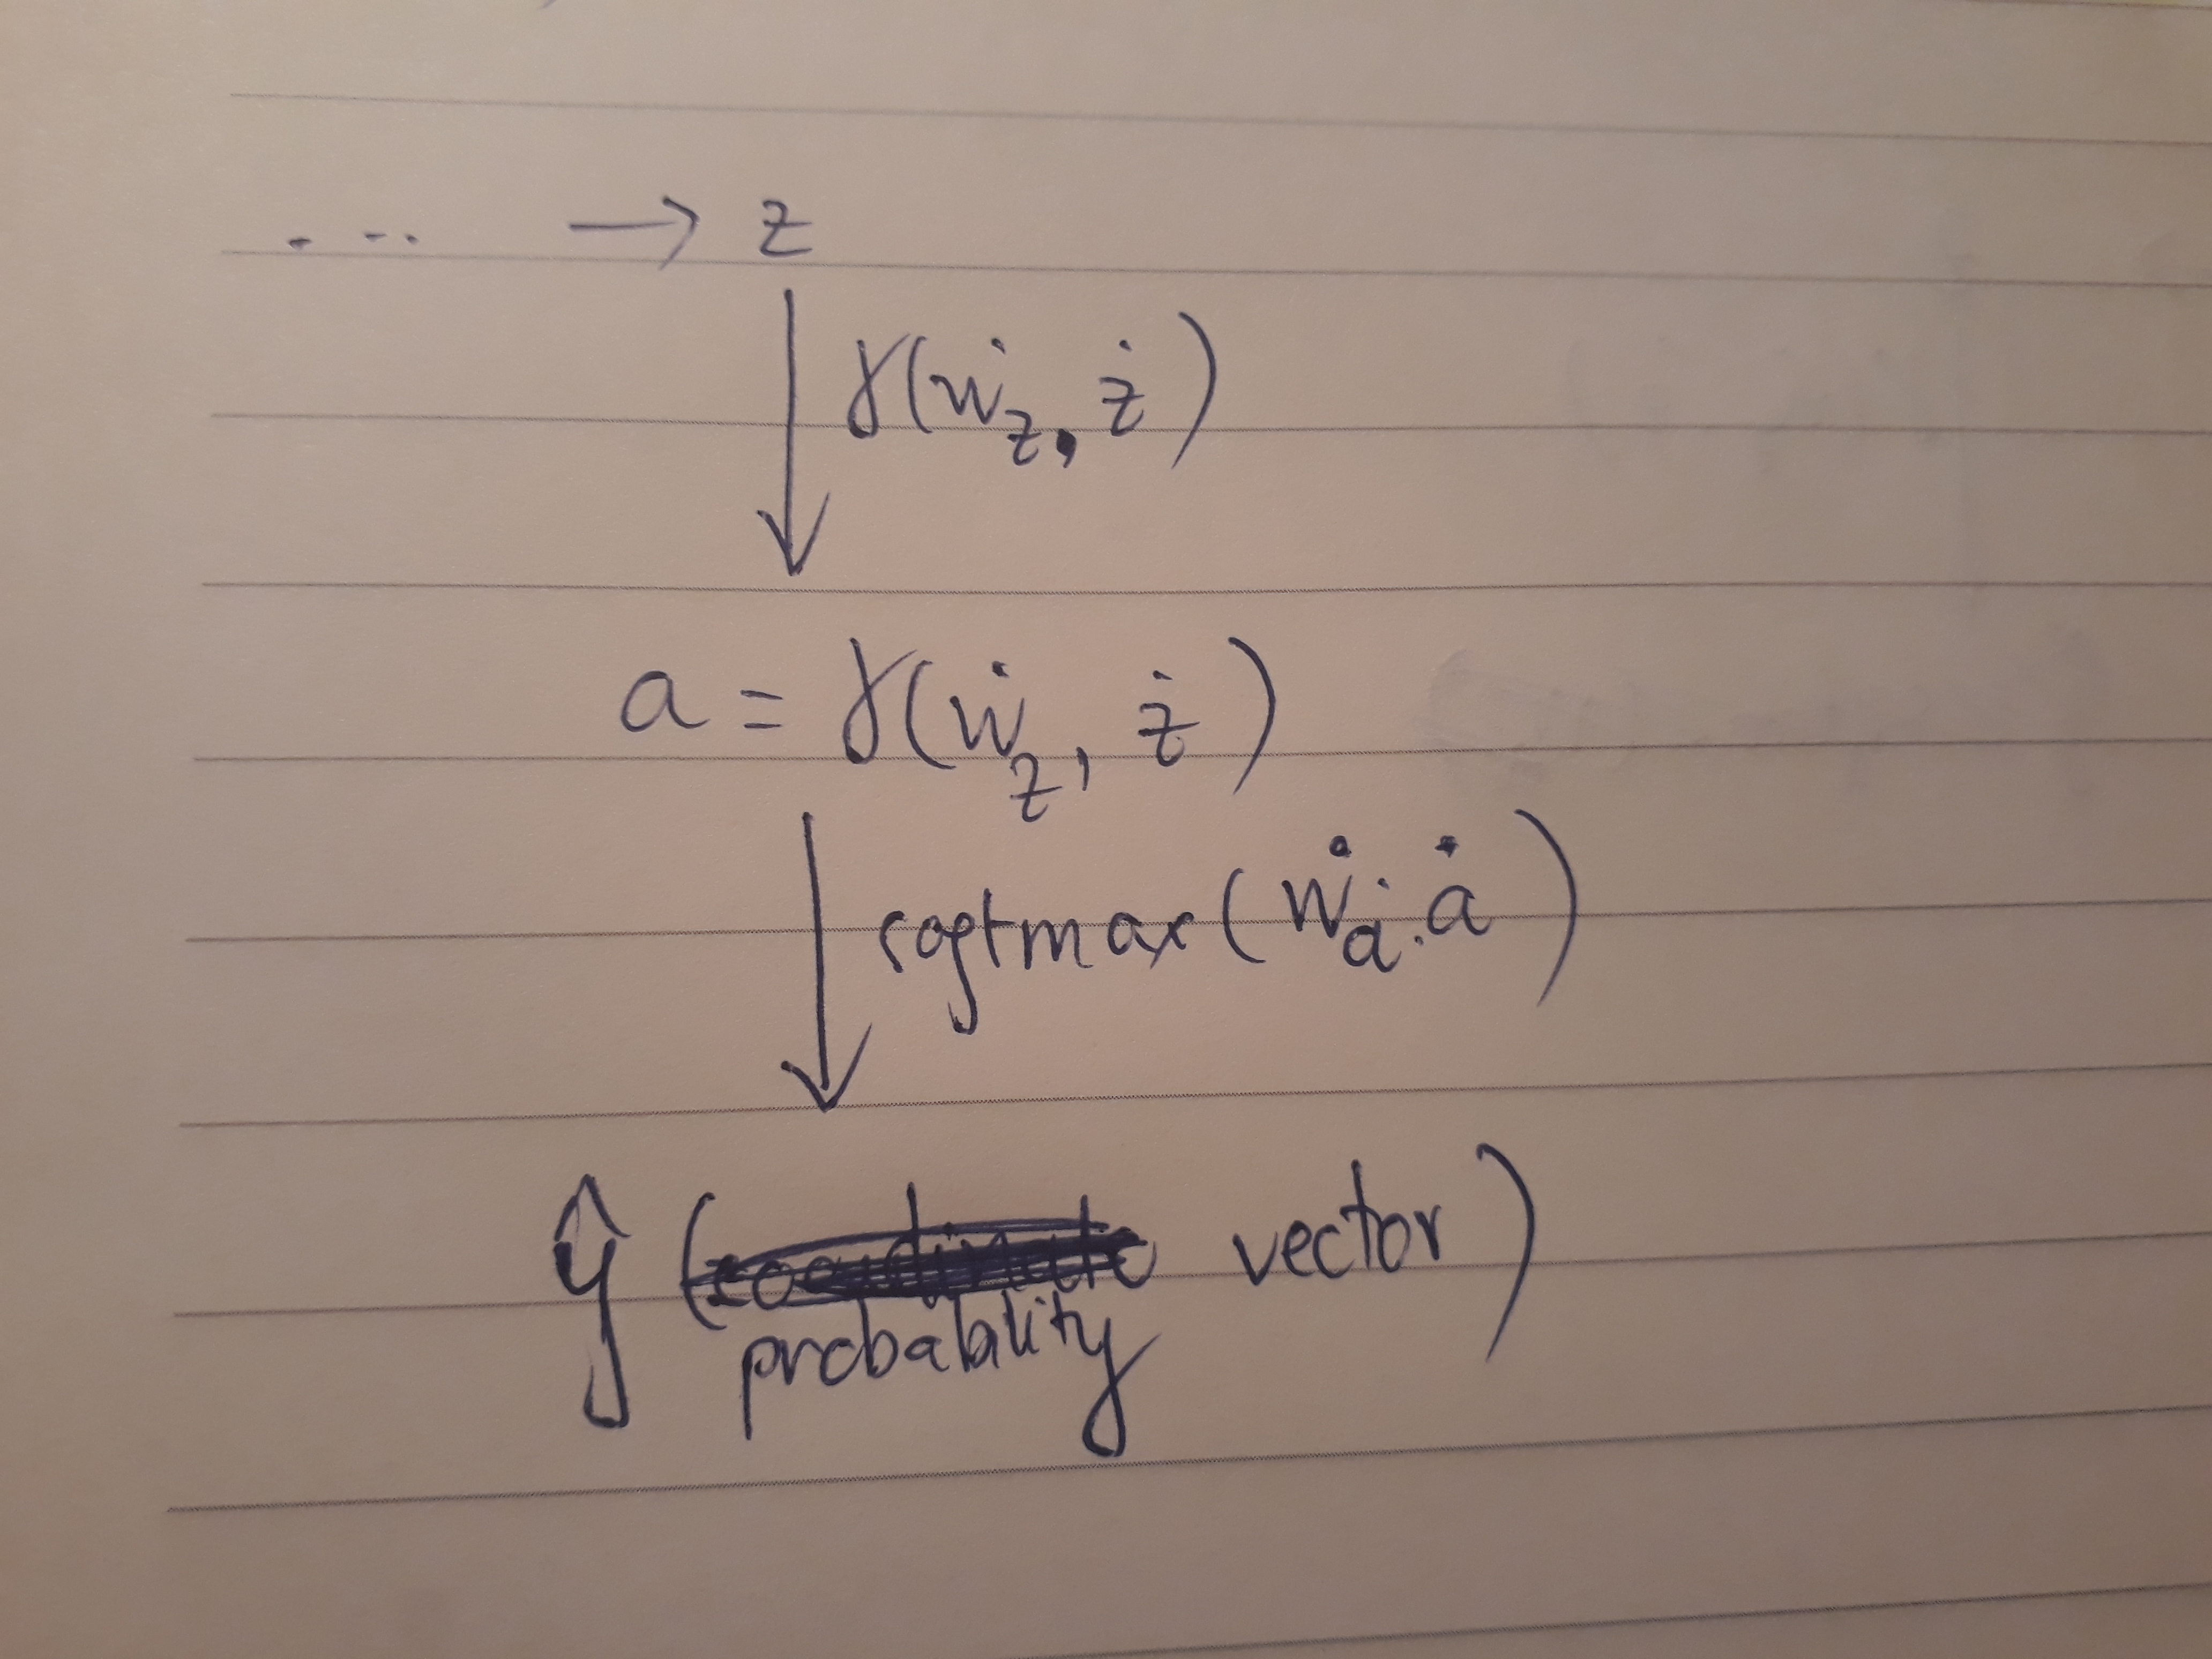
\includegraphics[scale=0.1]{20190703_013016.jpg}\\

\end{center}

\caption{Unified Framework - Multi-layer Regression}\\

- Từ z, tính a theo non-linear function -> Từ a tính probability vector $\hat{y}$ theo non-linear function tiếp theo (ở đây là softmax) \\ 
=> Sử dụng các phép tính này lặp đi lặp lại để vẽ được những đường cong phân chia những dữ liệu đã cho phức tạp và chính xác

\end{figure}
\end{document}
